% Գլուխ 3. Գործնական մաս (սևագիր v1). Աղյուսակները գեներացվում են src/make_tables.py-ով

\chapter{Գործնական մաս}

\section{Իրականացում}

Բոլոր ալգորիթմները իրականացված են Python~3 լեզվով (ռեպոզիտորիայի \texttt{src/} պանակ): \texttt{NetworkX} գրադարանը օգտագործվում է միայն գրաֆներ կառուցելու և \emph{արդյունքները ստուգելու} համար, իսկ հենց ալգորիթմները գրված են ձեռքով.
\begin{itemize}
  \item \texttt{connectivity.py}՝ BFS/DFS բաղադրիչներ, Տարյանի ալգորիթմ (կամուրջներ և կտրող կետեր), Էդմոնդս--Կարպի առավելագույն հոսք, կողային կապակցվածություն $\lambda$ և գագաթային կապակցվածություն $\kappa$ (գագաթների տրոհման եղանակով).
  \item \texttt{reliability.py}՝ լրիվ թվարկում, գործոնավորում, Monte Carlo սիմուլյացիա (DSU կառուցվածքով).
  \item \texttt{experiments.py}՝ այս գլխի բոլոր փորձերը, արդյունքները գրվում են \texttt{results/results.json} ֆայլում, աղյուսակները և գրաֆիկները գեներացվում են ավտոմատ:
\end{itemize}

\textbf{Ճշտության ստուգում.} \texttt{tests/test\_all.py} ֆայլի 7 թեստերը համեմատում են իրականացումը \texttt{NetworkX}-ի հետ 23 գրաֆի վրա (ուղի, ցիկլ, լրիվ գրաֆ, Պետերսենի գրաֆ, ցանց, բարբելի գրաֆ (barbell), 15 պատահական գրաֆ և այլն). ստուգվում են բաղադրիչները, կամուրջները, կտրող կետերը, $\lambda$ և $\kappa$ արժեքները, Ուիթնիի անհավասարությունը $\kappa\le\lambda\le\delta$, հուսալիության փակ բանաձևերը ծառի և ցիկլի համար (Օրինակ~\ref{ex:reliab}), գործոնավորման և թվարկման համընկնումը (ճշտությամբ $10^{-12}$) և Monte Carlo արդյունքի ընկնելը վստահության միջակայքում: Բոլոր թեստերն անցնում են:

\section{Փորձեր}

Փորձերը կատարվել են 5 մոդելային գրաֆների վրա՝ ցիկլ $C_8$, անիվ $W_7$, $3\times3$ քառակուսի ցանց, լրիվ գրաֆ $K_5$ և Պետերսենի գրաֆ: Բոլոր կողերն ունեն նույն $p$ աշխատունակության հավանականությունը, գագաթները բացարձակ հուսալի են (Գլուխ~1-ի մոդել):

\subsection{Կառուցվածքային պարամետրներ}

\begin{table}[h]
\centering
\small
\begin{tabular}{|l|c|c|c|c|c|c|c|}
\hline
Գրաֆ & $n$ & $m$ & $\delta$ & $\kappa$ & $\lambda$ & կամուրջներ & կտրող կետեր\\
\hline
Ցիկլ C8 & 8 & 8 & 2 & 2 & 2 & 0 & 0\\
\hline
Անիվ W7 & 7 & 12 & 3 & 3 & 3 & 0 & 0\\
\hline
Ցանց 3x3 & 9 & 12 & 2 & 2 & 2 & 0 & 0\\
\hline
Լրիվ K5 & 5 & 10 & 4 & 4 & 4 & 0 & 0\\
\hline
Պետերսեն & 10 & 15 & 3 & 3 & 3 & 0 & 0\\
\hline
\end{tabular}

\caption{Գրաֆների կառուցվածքային պարամետրները, հաշված ալգորիթմներով Գլուխ~2-ից}
\end{table}

Բոլոր 5 գրաֆներում $\kappa=\lambda=\delta$, այսինքն՝ Ուիթնիի անհավասարությունը (Գլուխ~1) այստեղ դառնում է հավասարություն, կամուրջներ և կտրող կետեր չկան: Սա սպասելի է այս սիմետրիկ գրաֆների համար, բայց ընդհանուր դեպքում $\kappa<\lambda<\delta$ հնարավոր է (օրինակ՝ երկու լրիվ գրաֆ, միացված մեկ գագաթով): Թեստերի պատահական գրաֆների վրա անհավասարությունը նույնպես բավարարվում է:

\subsection{Հուսալիության կախումը $p$-ից}

\begin{figure}[h]
\centering
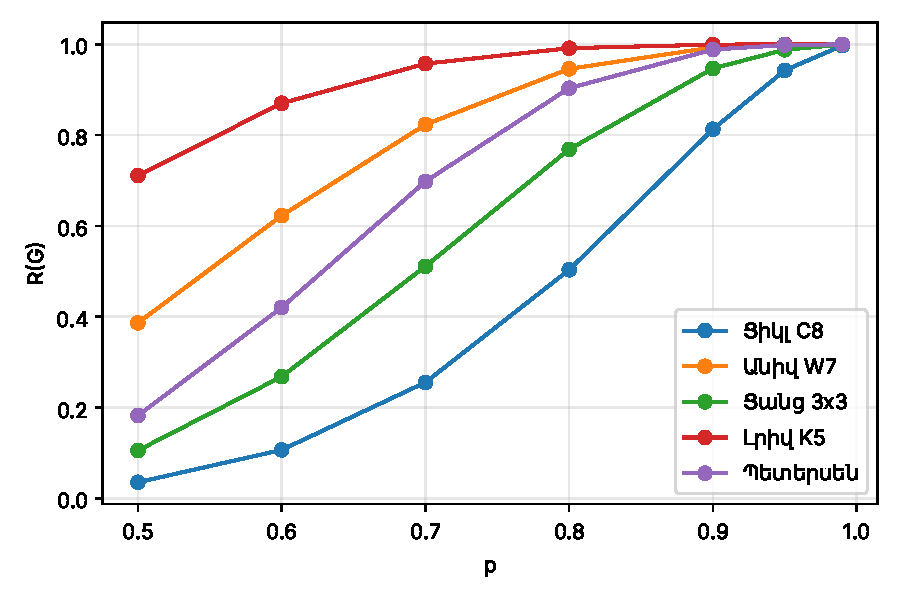
\includegraphics[width=0.8\textwidth]{figures/rel_vs_p.pdf}
\caption{$R(G)$ կախվածությունը կողի աշխատունակության $p$ հավանականությունից}
\end{figure}

\begin{table}[h]
\centering
\small
\begin{tabular}{|l|c|c|c|c|}
\hline
Գրաֆ & $p=0{,}50$ & $p=0{,}80$ & $p=0{,}90$ & $p=0{,}95$\\
\hline
Ցիկլ C8 & 0{,}0352 & 0{,}5033 & 0{,}8131 & 0{,}9428\\
\hline
Անիվ W7 & 0{,}3862 & 0{,}9461 & 0{,}9935 & 0{,}9992\\
\hline
Ցանց 3x3 & 0{,}1052 & 0{,}7688 & 0{,}9470 & 0{,}9882\\
\hline
Լրիվ K5 & 0{,}7109 & 0{,}9917 & 0{,}9995 & 1{,}0000\\
\hline
Պետերսեն & 0{,}1821 & 0{,}9035 & 0{,}9886 & 0{,}9987\\
\hline
\end{tabular}

\caption{Բոլոր գագաթների հուսալիությունը ընտրված $p$ արժեքների համար (ճշգրիտ, գործոնավորմամբ)}
\end{table}

Բոլոր $p$-երի համար գրաֆների դասավորությունը նույնն է. $K_5>W_7>$ Պետերսեն $>3\times3>C_8$: Մեծ $\lambda$-ով գրաֆները ավելի հուսալի են ($K_5$-ի համար $\lambda=4$, $C_8$-ի համար $\lambda=2$), իսկ նույն $\lambda=3$-ի դեպքում ($W_7$ և Պետերսեն) ավելի փոքր գրաֆը ($W_7$, 7 գագաթ) ավելի հուսալի է, որովհետև պետք է կապակցել ավելի քիչ գագաթներ: Տարբերությունը մեծ է. $p=0{,}9$ դեպքում $C_8$-ը կապակցված է մնում ժամանակի $81\%$-ում, իսկ $K_5$-ը՝ $99{,}95\%$-ում:

\subsection{Կապերի ավելացման ազդեցությունը}

Վերցնենք $C_8$ ցիկլը և ավելացնենք 1, ապա 2 լրացուցիչ կող՝ $\{0,4\}$ և $\{2,6\}$:

\begin{table}[h]
\centering
\small
\begin{tabular}{|l|c|c|}
\hline
Գրաֆ & $R$ ($p=0{,}7$) & $R$ ($p=0{,}9$)\\
\hline
C8 & 0{,}2553 & 0{,}8131\\
\hline
C8 + 1 լրաց. կող & 0{,}3739 & 0{,}8896\\
\hline
C8 + 2 լրաց. կող & 0{,}5221 & 0{,}9470\\
\hline
\end{tabular}

\caption{Լրացուցիչ կողերի ազդեցությունը $C_8$ ցիկլի հուսալիության վրա}
\end{table}

Երկու լրացուցիչ կողը $p=0{,}7$ դեպքում հուսալիությունը գրեթե կրկնապատկում է ($0{,}26\to0{,}52$): Հետաքրքիր է, որ $\lambda$-ն այս ընթացքում \emph{չի փոխվում} ($\lambda=2$, քանի որ $1,3,5,7$ գագաթները դեռ ունեն աստիճան 2), թեև հուսալիությունը զգալիորեն աճում է: Սա ցույց է տալիս, որ միայն կապակցվածության թիվը չի բնութագրում ցանցի հուսալիությունը. կարևոր է նաև, թե քանի կտրվածք ունի ցանցը փոքր չափի (տե՛ս բաժին~2.3.3):

\subsection{Կտրվածքային գնահատականներ}

\begin{table}[h]
\centering
\small
\begin{tabular}{|l|c|c|c|}
\hline
Գրաֆ & ստորին & ճշգրիտ $R$ & վերին\\
\hline
Ցիկլ C8 & 0{,}7130 & 0{,}8131 & 0{,}9900\\
\hline
Անիվ W7 & 0{,}9933 & 0{,}9935 & 0{,}9990\\
\hline
Ցանց 3x3 & 0{,}9411 & 0{,}9470 & 0{,}9900\\
\hline
Լրիվ K5 & 0{,}9995 & 0{,}9995 & 0{,}9999\\
\hline
Պետերսեն & 0{,}9880 & 0{,}9886 & 0{,}9990\\
\hline
\end{tabular}

\caption{Թեորեմ~\ref{thm:bounds}-ի գնահատականները, $p=0{,}9$}
\end{table}

Բոլոր դեպքերում ստորին $\le$ ճշգրիտ $\le$ վերին, ինչպես պահանջում է թեորեմը: Ստորին գնահատականը շատ մոտ է ճշգրիտ արժեքին այն գրաֆների համար, որտեղ փոքր կտրվածքները քիչ են ($K_5$, $W_7$, Պետերսեն). տարբերությունը $<0{,}001$: $C_8$-ի համար, որտեղ կան բազմաթիվ 2 կողանի կտրվածքներ, ստորին գնահատականը աղոտ է ($0{,}713$ ընդդեմ $0{,}813$): Վերին գնահատականը (որը օգտագործում է միայն $\lambda$-ն) կոպիտ է, հատկապես փոքր $\lambda$-ի դեպքում:

\subsection{Ճշգրիտ մեթոդներ և Monte Carlo. արագություն և ճշտություն}

Համեմատենք երեք մեթոդները $W_k$ անիվ-գրաֆների վրա ($p=0{,}9$, $m=2(k-1)$ կող). Monte Carlo-ի համար օգտագործվել է $N=20000$ փորձ:

\begin{figure}[h]
\centering
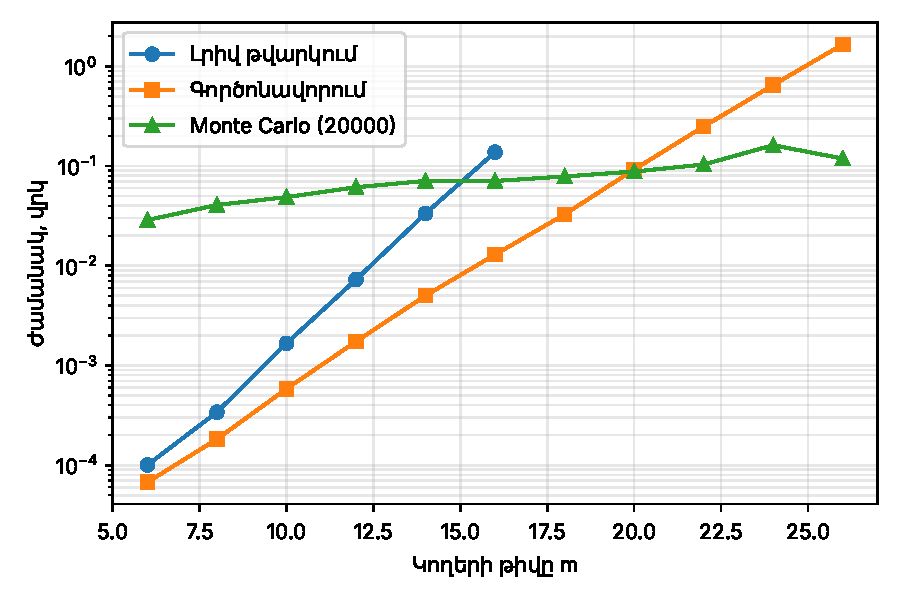
\includegraphics[width=0.8\textwidth]{figures/timing.pdf}
\caption{Մեթոդների աշխատանքի ժամանակը կողերի թվի կախվածությամբ (լոգարիթմական սանդղակ)}
\end{figure}

\begin{table}[h]
\centering
\small
\begin{tabular}{|c|c|c|c|c|c|c|}
\hline
$m$ & թվարկում, վրկ & գործոն., վրկ & MC, վրկ & $R$ ճշգրիտ & $R$ MC & 95\% միջակայք\\
\hline
6 & 0{,}0001 & 0{,}0001 & 0{,}0287 & 0{,}99581 & 0{,}99605 & $\pm$0{,}0009\\
\hline
8 & 0{,}0003 & 0{,}0002 & 0{,}0406 & 0{,}99557 & 0{,}99555 & $\pm$0{,}0009\\
\hline
10 & 0{,}0017 & 0{,}0006 & 0{,}0488 & 0{,}99456 & 0{,}99480 & $\pm$0{,}0010\\
\hline
12 & 0{,}0073 & 0{,}0017 & 0{,}0612 & 0{,}99349 & 0{,}99320 & $\pm$0{,}0011\\
\hline
14 & 0{,}0335 & 0{,}0050 & 0{,}0709 & 0{,}99241 & 0{,}99220 & $\pm$0{,}0012\\
\hline
16 & 0{,}1376 & 0{,}0129 & 0{,}0707 & 0{,}99133 & 0{,}99035 & $\pm$0{,}0014\\
\hline
18 & -- & 0{,}0327 & 0{,}0786 & 0{,}99025 & 0{,}99065 & $\pm$0{,}0013\\
\hline
20 & -- & 0{,}0921 & 0{,}0879 & 0{,}98917 & 0{,}98995 & $\pm$0{,}0014\\
\hline
22 & -- & 0{,}2486 & 0{,}1035 & 0{,}98809 & 0{,}98965 & $\pm$0{,}0014\\
\hline
24 & -- & 0{,}6491 & 0{,}1616 & 0{,}98702 & 0{,}98875 & $\pm$0{,}0015\\
\hline
26 & -- & 1{,}6576 & 0{,}1186 & 0{,}98594 & 0{,}98590 & $\pm$0{,}0016\\
\hline
\end{tabular}

\caption{Ժամանակը և արդյունքը ($p=0{,}9$, $N=20000$). «--»՝ չի չափվել ($m>16$)}
\end{table}

Դիտարկումները.
\begin{itemize}
  \item Լրիվ թվարկումը աճում է մոտավորապես 4 անգամ ամեն 2 նոր կողի համար ($2^2$) և $m=16$ դեպքում արդեն տևում է $\approx0{,}14$ վրկ: Էքստրապոլյացիայով $m=26$ դեպքում դա կլիներ $\approx2$ րոպե, իսկ $m=40$ դեպքում՝ շուրջ մեկ ամիս, ուստի $m>16$ համար թվարկումը չի չափվել:
  \item Գործոնավորումը նույն $m$-երի համար մոտ 10 անգամ արագ է թվարկումից ($m=16$. $0{,}013$ ընդդեմ $0{,}138$ վրկ) շնորհիվ վաղ էտման, բայց նրա ժամանակն էլ է աճում էքսպոնենցիալ ($m=26$. $\approx1{,}7$ վրկ):
  \item Monte Carlo-ի ժամանակը աճում է մոտավորապես գծային ($0{,}03\to0{,}12$ վրկ $m=6\to26$ դեպքում, չափումները աղմկոտ են): Գործոնավորման և Monte Carlo-ի ժամանակները հավասարվում են $m\approx20$ դեպքում ($\approx0{,}09$ վրկ երկուսի համար). $m=22$ դեպքում գործոնավորումը $0{,}25$ ընդդեմ $0{,}10$ վրկ է, իսկ $m=26$ դեպքում՝ $\approx14$ անգամ դանդաղ:
  \item Monte Carlo-ի 95\% միջակայքը ($\approx\pm0{,}001$--$0{,}0016$) պարունակել է ճշգրիտ արժեքը 11 դեպքից 9
-ում: Մնացած դեպքերում շեղումը մի փոքր գերազանցել է միջակայքը (մինչև $1{,}2$ անգամ). նկատենք, որ բոլոր չափումների համար օգտագործվել է նույն սերմը (\texttt{seed=3}), ուստի սխալները միմյանցից անկախ չեն:
\end{itemize}

\subsection{Monte Carlo-ի սխալի կախումը փորձերի թվից}

$3\times3$ ցանցի համար ($p=0{,}8$, ճշգրիտ $R=0{,}7688$) $N$-ի տարբեր արժեքներով 10 անկախ սերմերով հաշվվել է միջին բացարձակ սխալը:

\begin{figure}[h]
\centering
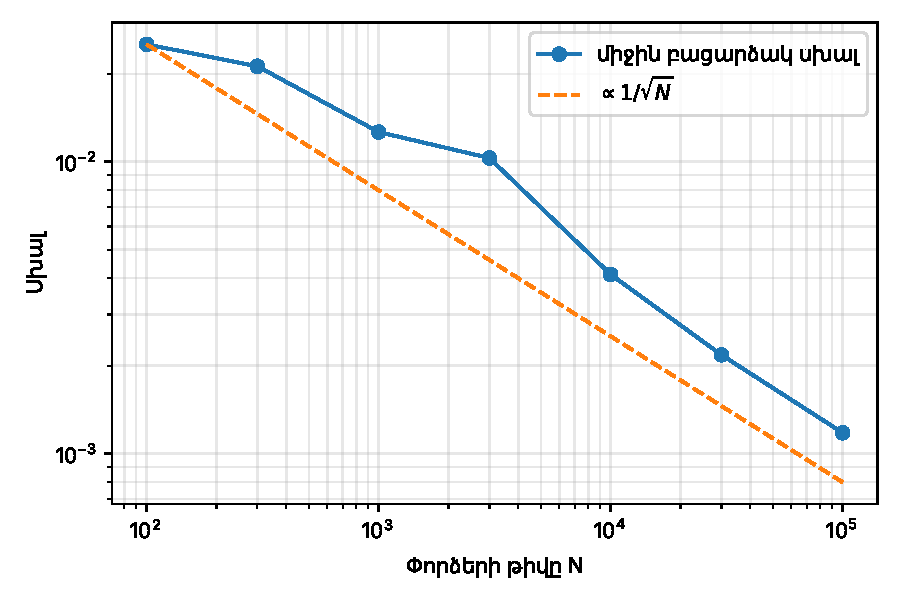
\includegraphics[width=0.8\textwidth]{figures/mc_error.pdf}
\caption{Monte Carlo-ի սխալը՝ ըստ $N$-ի (լոգարիթմական սանդղակ), կետագիծը՝ $1/\sqrt N$ կախվածությունը}
\end{figure}

\begin{table}[h]
\centering
\small
\begin{tabular}{|r|c|}
\hline
$N$ & միջին $|\widehat R_N-R|$\\
\hline
100 & 0{,}02524\\
\hline
300 & 0{,}02124\\
\hline
1000 & 0{,}01264\\
\hline
3000 & 0{,}01030\\
\hline
10000 & 0{,}00411\\
\hline
30000 & 0{,}00218\\
\hline
100000 & 0{,}00118\\
\hline
\end{tabular}

\caption{Monte Carlo-ի միջին բացարձակ սխալը}
\end{table}

$N$-ը 1000 անգամ մեծացնելիս ($100\to10^5$) սխալը փոքրացել է մոտ 21 անգամ, ինչը մոտ է տեսականին՝ $\sqrt{1000}\approx32$ (միջինացումը ընդամենը 10 սերմի վրա է, այդ պատճառով կորը աղմկոտ է): Եզրակացությունը համապատասխանում է Բաժին~2.4-ի. սխալը նվազում է $1/\sqrt N$ արագությամբ:

\section{Ամփոփում}

Փորձերը հաստատում են տեսական եզրակացությունները.
\begin{enumerate}
  \item ճշգրիտ մեթոդները (թվարկում, գործոնավորում) տալիս են նույն արդյունքը և կիրառելի են $m\lesssim25$ կողի համար, դրանից հետո ժամանակը աճում է էքսպոնենցիալ.
  \item Monte Carlo-ն ունի գծային բարդություն և հնարավորություն է տալիս գնահատել մեծ գրաֆները, սակայն ճշտությունը լավացնելու գինը $N\propto1/\varepsilon^2$ է.
  \item կապակցվածության չափանիշները ($\lambda$, $\kappa$) և հուսալիությունը կապված են, բայց հուսալիությունը կախված է նաև կտրվածքների թվից (օրինակ՝ լրացուցիչ կող ավելացնելը $\lambda$-ն չփոխելով բարձրացնում է $R$-ը).
  \item կտրվածքային գնահատականները շատ ճշգրիտ են բարձր $p$-ի և քիչ փոքր կտրվածքներով գրաֆների համար:
\end{enumerate}

\textbf{Սահմանափակումներ.} Փորձարկումը կատարվել է փոքր մոդելային գրաֆների վրա, բոլոր կողերը ունեն նույն $p$ և գագաթները չեն խափանվում: Իրական ցանցերի (օրինակ՝ մայրուղային կամ հաղորդակցական ցանցերի տոպոլոգիաներ) վրա փորձարկումը և գագաթային խափանումների մոդելը կարող են ավելացվել հետագա աշխատանքում:
